\subsection{Running flexible PCB coils}

\subsubsection{High current needs}
As discussed in the previous paragraph flexible coils have very high resistance so to produce even low magnetic fields high current must be provided.
Considering the power limit of the Flexar coil $P_{max} = 0.8W$ we can calculate the maximum current that can be provided to the coil with \ref{eq:Joule_heating} as
\begin{equation}
    I = \sqrt{\frac{P_{max}}{R}} = \sqrt{\frac{0.8}{30}} = 0.1633A
\end{equation}

This value of current is pretty high for standard AC circuits based on operational amplifiers.
Op amps usually have a maximum output current of some tens of milliamps.
An option to power these coils could be to use premade audio amplifiers, but this would limit their working frequency range as audio amplifiers are designed to work in the audible frequency range which is about 20Hz to 20kHz.
Meanwhile, as this research's goal is to apply this technology to haptic applications we have to consider that the human tactile perception range is from sub 1Hz to 1kHz. % TODO: check these values
So the coils must be able to work in this frequency range.

The solution is to use a special type of Op Amps called power Op Amps, these devices are designed to provide high current outputs.
They are usually designed as simple op-amps with a power stage at the output.
\begin{figure}
    \centering
    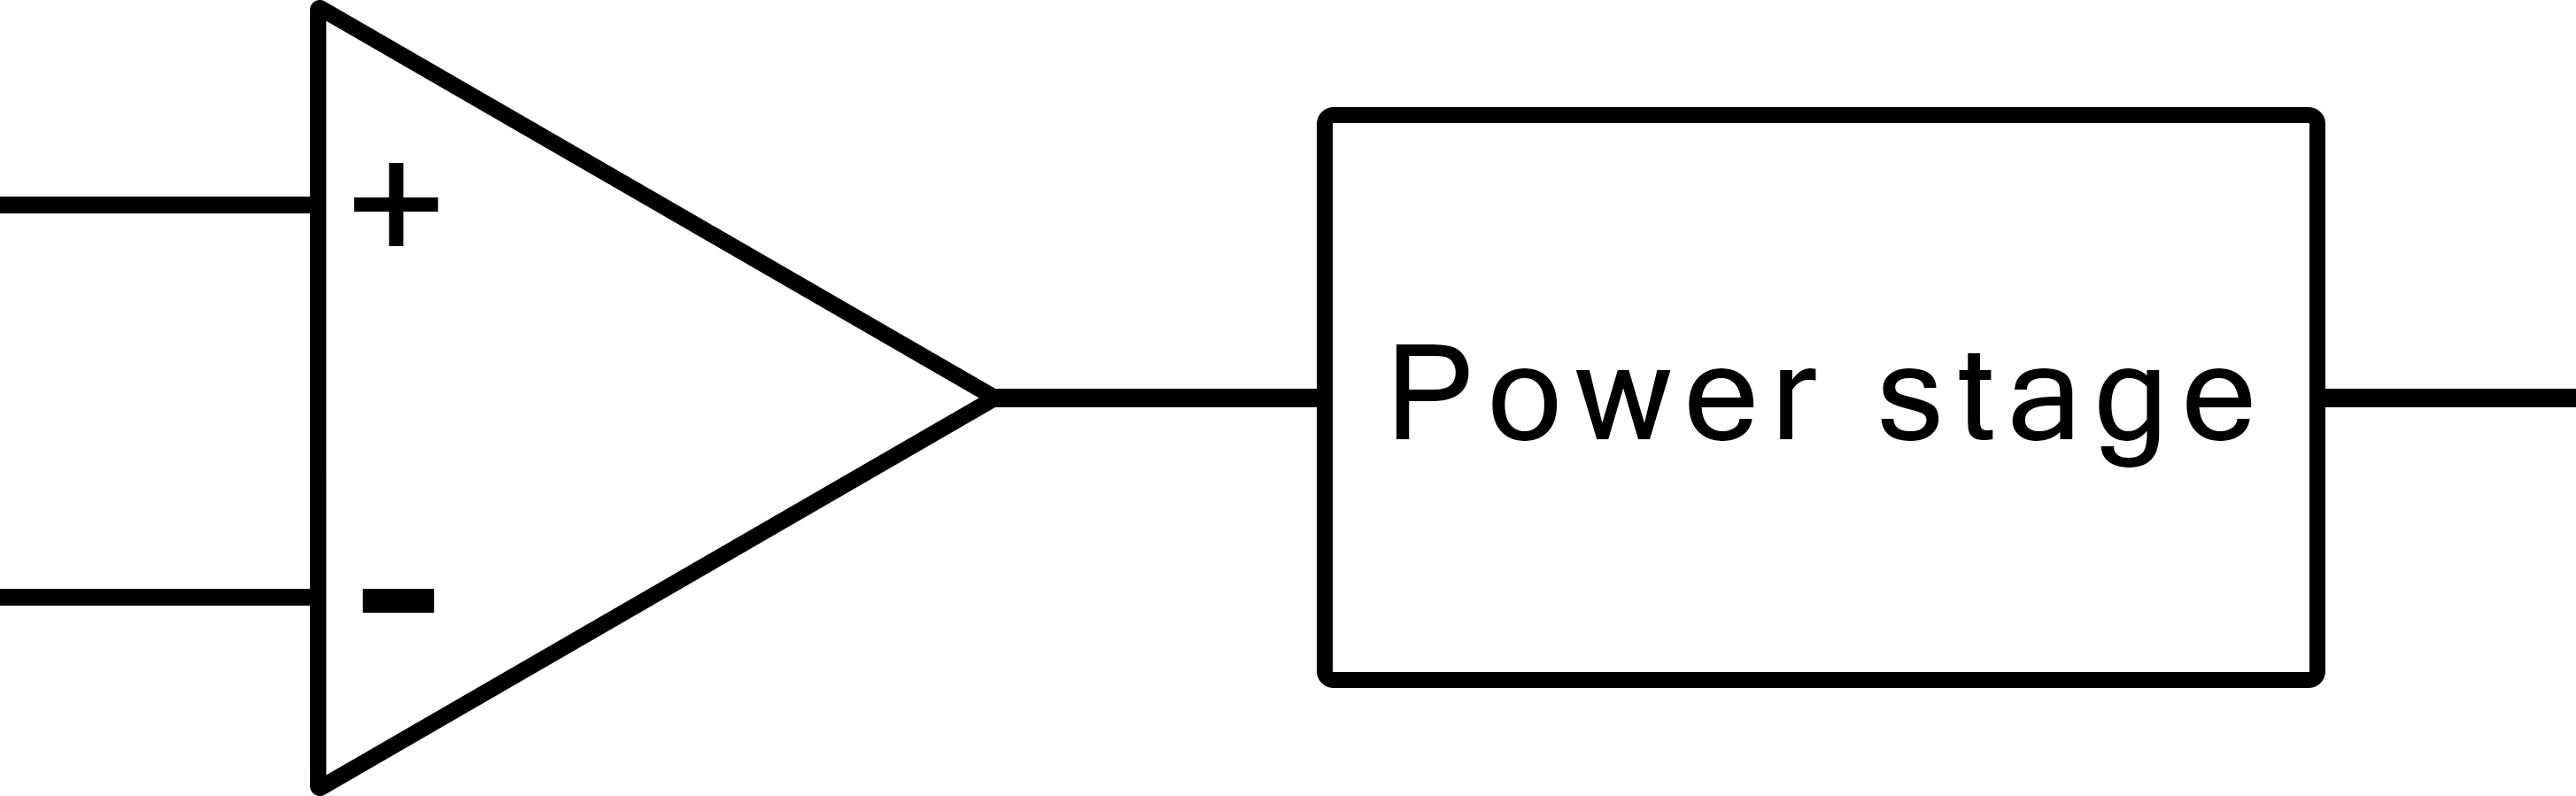
\includegraphics[width=0.5\textwidth]{Chapters/Chapter2/Flexible_PCB_Coils/Figures/power_op-amp_block_diagram.png}
    \caption{Power Op Amp block diagram.}
    \label{fig:Power_Op_Amp}
\end{figure}

\begin{figure}
    \vfill
    \includesvg[draft = false, width = 1\textwidth]{Chapters/Chapter2/Flexible_PCB_coils/Figures/power_op-amp_example.svg}
    \caption[Power op-amp schematic]{Example schematic of a power op-amp with a Class-AB power stage.}
    \label{fig:Power_op-amp_example}
\end{figure}

The Power op-amp we used in this research is the L272 from STMicroelectronics, it has a maximum output current of 1A with the capability to achieve 1.5A peak current (not continuously).
Also, it has a gain bandwidth product of 350kHz which is plenty enough for the application. \cite{L272}

\subsubsection{Constant Voltage vs Constant Current power supplying}
To power our coil we have two options, we can either provide a constant voltage or a constant current.
Using a constant current source is not advisable due to the heating problem of the coil, at high currents as the coil is run it will heat up and its resistance will increase which will cause the power source to increase the voltage to keep the current constant.
This in turn will cause the coil to heat up even more and the cycle will continue until the coil is damaged.

Instead, using a constant voltage source as the resistance increases due to the coil exceeding the heating and power threshold we will only have a decrease in the current which results in a loss of magnetic field strength but the coil won't get damaged.

